% Finite-Elemente (ZHAW) — Beamer-Template
% (Passe Titel/Dozent/Datum nach Bedarf an.)

\documentclass[aspectratio=169,professionalfonts]{beamer}

% --- Sprache/Encoding ---
\usepackage[ngerman]{babel}
\usepackage[T1]{fontenc}
\usepackage[utf8]{inputenc}

% --- Mathe & Grafik ---
\usepackage{amsmath,amssymb,bm}
\usepackage{mathtools}
\usepackage{graphicx}
\usepackage{tikz}
\usetikzlibrary{arrows.meta,positioning,calc,decorations.pathmorphing,matrix,fit}
\pgfdeclarelayer{background}
\pgfsetlayers{background,main}

% --- Tabellen/Listen ---
\usepackage{booktabs}
\usepackage{multicol}

% --- Theme/Look ---
\usetheme{Madrid}
\usecolortheme{default}
\setbeamertemplate{navigation symbols}{}

% Fußzeile: Foliennummern
\setbeamertemplate{footline}{%
  \leavevmode%
  \hbox{%
  \begin{beamercolorbox}[wd=.8\paperwidth,ht=2.5ex,dp=1.1ex,left]{author in head/foot}\hspace{1em}\insertshortauthor\hspace{1em}--\hspace{1em}\insertshorttitle\end{beamercolorbox}%
  \begin{beamercolorbox}[wd=.2\paperwidth,ht=2.5ex,dp=1.1ex,right]{date in head/foot}\insertframenumber{} / \inserttotalframenumber\hspace{1em}\end{beamercolorbox}}%
  \vskip0pt%
}

% --- Metadaten ---
\title[FEM]{Finite Elemente Methode}
\subtitle{Vorlesung}
\author[ZHAW]{Sebastian Domaschke}
\institute[ZHAW]{Zürcher Hochschule für Angewandte Wissenschaften (ZHAW)}
\date{Frühlingssemester 2026}
\titlegraphic{
\includegraphics[height=1.2cm]{../Grafiken/logo.pdf}}

% --- Nützliche Makros ---
\newcommand{\R}{\mathbb{R}}
\newcommand{\dd}{\,\mathrm{d}}
\newcommand{\grad}{\nabla}
\newcommand{\K}{\mathbf{K}}
\newcommand{\fvec}{\mathbf{f}}
\newcommand{\uvec}{\mathbf{u}}

\begin{document}

% Titelfolie
\begin{frame}
  \titlepage
\end{frame}


\newsavebox{\FachwerkPic}
\sbox{\FachwerkPic}{%
\begin{tikzpicture}[scale=0.95, every node/.style={font=\small},
  disp/.style={draw=green!70!black, very thick, -{Latex[length=3mm]}, green!70!black},
  load/.style={draw=red!80!black, very thick, -{Latex[length=3mm]}, red!80!black},
  member/.style={line width=1.2pt, black},
  joint/.style={circle, fill=black, inner sep=2.2pt},
  elbox/.style={draw, rectangle, inner sep=2pt, fill=white}
]
  % Knoten
  \coordinate (n1) at (0,0);
  \coordinate (n2) at (4,0);
  \coordinate (n3) at (4,3);
  \coordinate (n4) at (8,3);

  % Stäbe (Elemente)
  \draw[member] (n1) -- (n2); % e1
  \draw[member] (n1) -- (n3); % e2
  \draw[member] (n2) -- (n3); % e3
  \draw[member] (n2) -- (n4); % e4
  \draw[member] (n3) -- (n4); % e5

  % Gelenke
  \node[joint] at (n1) {};
  \node[joint] at (n2) {};
  \node[joint] at (n3) {};
  \node[joint] at (n4) {};

  % Knotennummern
  \node[above left] at (n1) {$1$};
  \node[above left] at (n2) {$2$};
  \node[above left] at (n3) {$3$};
  \node[above left] at (n4) {$4$};

  % Elementnummern
  \node[elbox] at (2.0,-0.35) {$1$};
  \node[elbox] at (1.8,1.45) {$2$};
  \node[elbox] at (4.25,1.5) {$3$};
  \node[elbox] at (6.0,1.35) {$4$};
  \node[elbox] at (6.0,3.25) {$5$};

  % Lager
  \draw[line width=1pt] (n1) ++(-0.35,-0.35) -- ++(0.70,0) ;
  \draw[line width=1pt] (n1) ++(-0.35,-0.35) -- (n1);
  \draw[line width=1pt] (n1) ++(0.35,-0.35) -- (n1);
  \foreach \xx in {-0.40,-0.28,...,0.40} {\draw (n1) ++(\xx,-0.35) -- ++(0.12,-0.12);}

  \draw[line width=1pt] (n2) ++(-0.35,-0.35) -- ++(0.70,0) ;
  \draw[line width=1pt] (n2) ++(-0.35,-0.35) -- (n2);
  \draw[line width=1pt] (n2) ++(0.35,-0.35) -- (n2);
  \foreach \xx in {-0.40,-0.28,...,0.40} {\draw (n2) ++(\xx,-0.35) -- ++(0.12,-0.12);}

  % Verschiebungen (grün)
  \draw[disp] (n1) -- ++(1.1,0) node[below right] {$U_1$};
  \draw[disp] (n1) -- ++(0,1.1) node[left] {$U_2$};

  \draw[disp] (n2) -- ++(1.1,0) node[below right] {$U_3$};
  \draw[disp] (n2) -- ++(0,1.1) node[left] {$U_4$};

  \draw[disp] (n3) -- ++(1.1,0) node[above] {$U_5$};
  \draw[disp] (n3) -- ++(0,1.1) node[left] {$U_6$};

  \draw[disp] (n4) -- ++(1.1,0) node[above] {$U_7$};
  \draw[disp] (n4) -- ++(0,1.1) node[left] {$U_8$};

  % Last (rot)
  \draw[load] (n4) -- ++(0,-1.4) node[right] {$F$};

  % Koordinatensystem
  \draw[->,thick] (6.8,0.1) -- ++(1.0,0) node[right] {$X$};
  \draw[->,thick] (6.8,0.1) -- ++(0,1.0) node[above] {$Y$};
\end{tikzpicture}%
}

\begin{frame}{Übergeordnetes Lernziel 2}
  \centering
  \begin{minipage}{0.9\linewidth}
    \centering
    {\LARGE  Herleitung / Erklärung FEM\\[0.6em]}
    {\Large bestehend aus 1D-Elementen (Federn, Stäben, Balken)\\[0.4em]}
    {\Large mittels \textbf{Matrixsteifigkeitsmethode}}
  \end{minipage}
\end{frame}

\begin{frame}{Lernziele Vorlesung}
  \small
  Sie können
  \begin{enumerate}
    \item Elementverschiebungen und Elementkräfte vom lokalen ins globale System transformieren.
        \item die Elementsteifigkeitsmatrix vom lokalen
ins globale System transformieren
            \item die
Koinzidenztabelle aufstellen
\item die Elementsteifigkeitsmatrizen zur
Struktursteifigkeitsmatrix zusammenbauen 
  \end{enumerate}
\end{frame}
\begin{frame}{Tafelbild (Wiederholung Lokale zu Globale Elementsteifigkeitsmatrix)}
  \centering
\end{frame}
\begin{frame}{Globale Elementsteifigkeitsmatrix (2D-Stab)}
  \small
  \begin{itemize}
    \item \textbf{Globale Elementsteifigkeitsmatrix} $\mathbf{K}^e$ (Transformation lokal $\rightarrow$ global)
  \end{itemize}

  \vspace{0.2em}
  \begin{block}{Transformation}
    $$\mathbf{K}^e = (\mathbf{T}^e)^{\mathsf T}\,\mathbf{k}^e\,\mathbf{T}^e$$
  \end{block}

  \vspace{0.3em}
  \begin{columns}[T,onlytextwidth]
    \begin{column}{0.60\textwidth}
      \scriptsize
      Mit $c=\cos\alpha^e$ und $s=\sin\alpha^e$:
      $$\mathbf{k}^e=\frac{E^eA^e}{L^e}
      \begin{pmatrix}
        1 & -1\\
        -1 & 1
      \end{pmatrix}$$

      $$\mathbf{T}^e=
      \begin{pmatrix}
        c & s & 0 & 0\\
        0 & 0 & c & s
      \end{pmatrix}$$

      \colorbox{blue!10}{$\displaystyle
      \mathbf{K}^e(\alpha^e)=\frac{E^eA^e}{L^e}
      \begin{pmatrix}
        c^2 & cs & -c^2 & -cs\\
        cs & s^2 & -cs & -s^2\\
        -c^2 & -cs & c^2 & cs\\
        -cs & -s^2 & cs & s^2
      \end{pmatrix}$}
    \end{column}
    \begin{column}{0.40\textwidth}
      \centering
      % TODO: PNG einfügen (statt TikZ)
      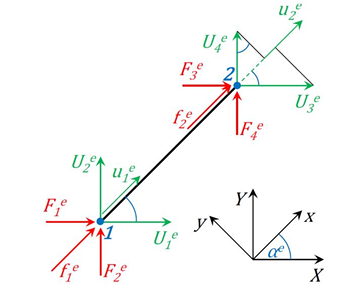
\includegraphics[width=\linewidth,height=0.55\textheight,keepaspectratio]{../Grafiken/V2_GlobaleElementmatrix.png}
    \end{column}
  \end{columns}
\end{frame}

\begin{frame}{Echte Probleme: Systeme aus mehreren Elementen (z.B. Fachwerk)}
  \centering
  \usebox{\FachwerkPic}
\end{frame}


\begin{frame}{Idee: Assemblierung - Globale Systemsteifigkeit aus Elementsteifigkeiten}
  \centering
  % TODO: Bitte das bereitgestellte Bild als Datei nach \texttt{../Grafiken/Assemblierung-Zyklus.png} hochladen
  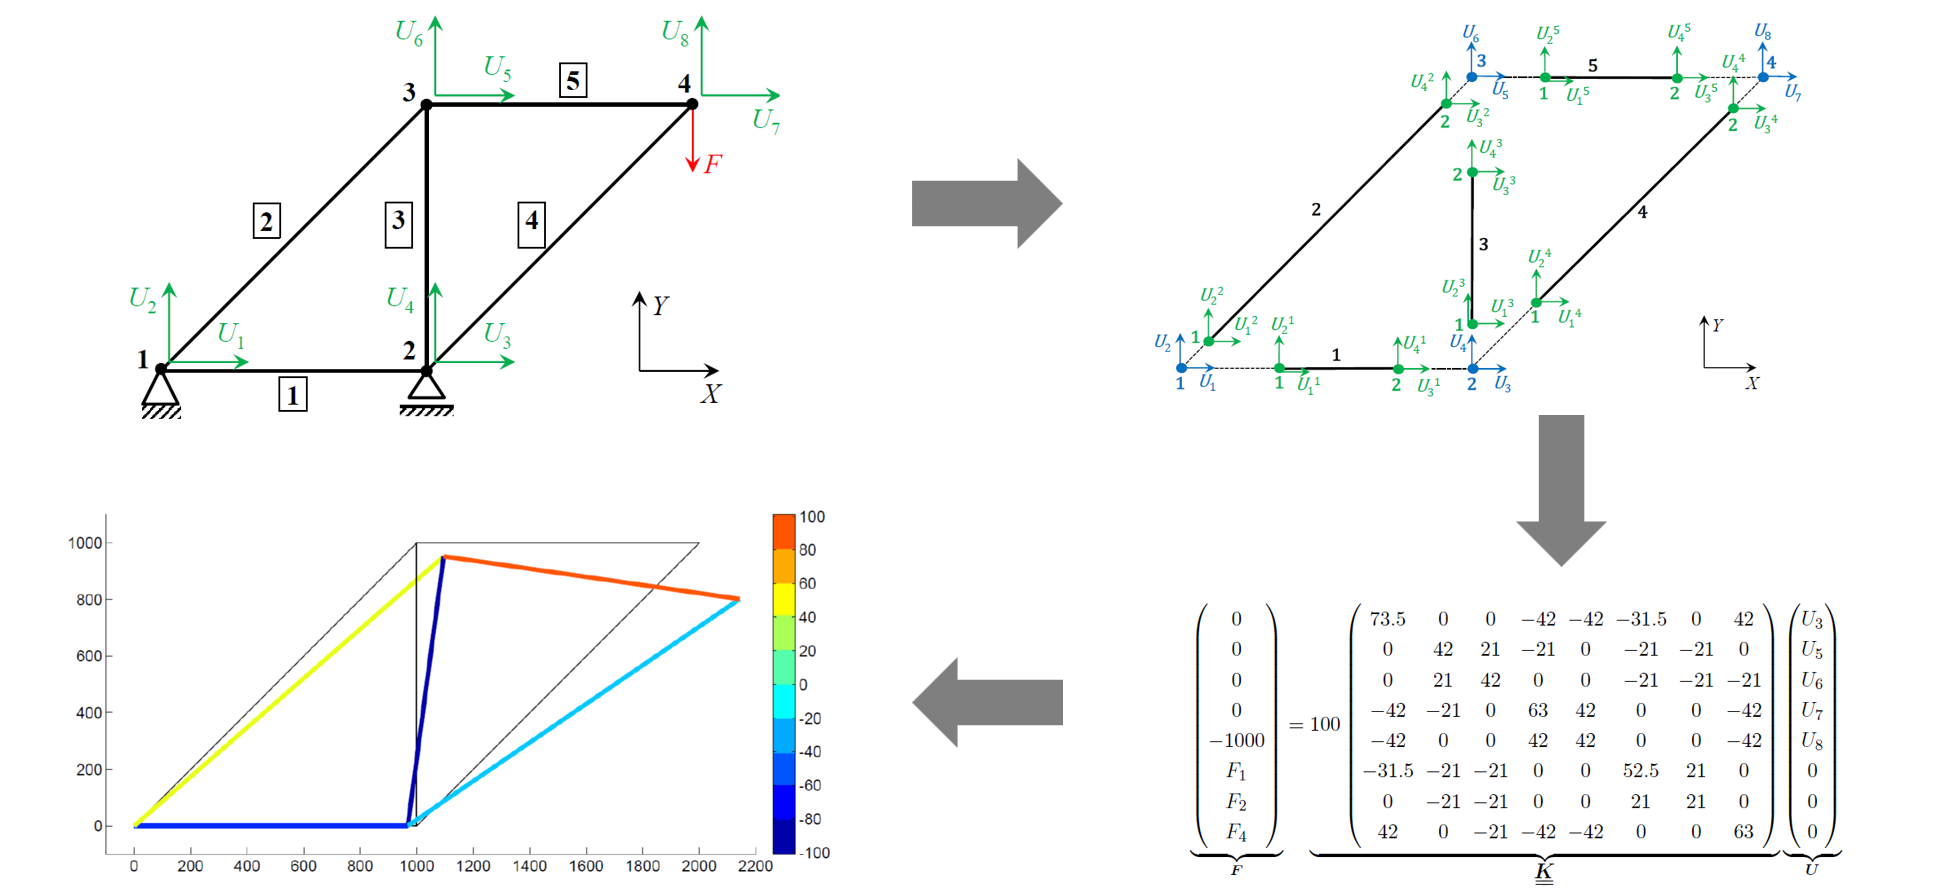
\includegraphics[width=0.98\linewidth,height=0.80\textheight,keepaspectratio]{../Grafiken/Assemblierung-Zyklus.png}
\end{frame}



\begin{frame}{Beispiele: Koinzidenztabellen}
  \small
  \begin{columns}[T,onlytextwidth]
    % --- Navier ---
    \begin{column}{0.49\textwidth}
      \centering
      {\large Navier's Problem}

      \vspace{0.4em}

      \begin{tikzpicture}[scale=0.82, every node/.style={font=\scriptsize},
        member/.style={line width=1.2pt, black},
        joint/.style={circle, fill=blue!70!black, inner sep=1.6pt},
        elbox/.style={draw, rectangle, inner sep=1.2pt, fill=white},
        support/.style={line width=0.9pt}
      ]
        % Fixe Bounding-Box (damit Lager/Tabellen in beiden Spalten auf gleicher Höhe sind)
        \useasboundingbox (-0.8,-0.7) rectangle (7.2,3.2);

        % Knoten
        \coordinate (n1) at (0,0);
        \coordinate (n2) at (1.6,0);
        \coordinate (n3) at (3.2,0);
        \coordinate (n4) at (4.8,0);
        \coordinate (n5) at (6.4,0);
        \coordinate (n6) at (3.2,2.8);

        % Stäbe (Elemente)
        \draw[member] (n6) -- (n1);
        \draw[member] (n6) -- (n2);
        \draw[member] (n6) -- (n3);
        \draw[member] (n6) -- (n4);
        \draw[member] (n6) -- (n5);

        % Elementnummern
        \node[elbox] at (1.45,1.05) {1};
        \node[elbox] at (2.15,1.25) {2};
        \node[elbox] at (3.2,1.35) {3};
        \node[elbox] at (4.25,1.25) {4};
        \node[elbox] at (4.95,1.05) {5};

        % Gelenke + Knotennummern
        \node[joint] at (n1) {}; \node[blue!70!black, above] at (n1) {1};
        \node[joint] at (n2) {}; \node[blue!70!black, above] at (n2) {2};
        \node[joint] at (n3) {}; \node[blue!70!black, above left] at (n3) {3};
        \node[joint] at (n4) {}; \node[blue!70!black, above ] at (n4) {4};
        \node[joint] at (n5) {}; \node[blue!70!black, above] at (n5) {5};
        \node[joint] at (n6) {}; \node[blue!70!black, above] at (n6) {6};

        % Lager (stilisierte Dreiecksauflager)
        \foreach \n in {n1,n2,n3,n4,n5} {%
          % Dreieck
          \draw[support] (\n) -- ++(-0.22,-0.22) -- ++(0.44,0) -- cycle;
          % Fundamentlinie + Schraffur
          \draw[support] (\n) ++(-0.35,-0.25) -- ++(0.70,0);
          \foreach \xx in {-0.35,-0.25,...,0.35} {\draw[support] (\n) ++(\xx,-0.25) -- ++(0.10,-0.10);}%
        }
      \end{tikzpicture}

      \vspace{0.6em}

      \scriptsize
      \begin{tabular}{c|ccccc}
        $e$ & 1 & 2 & 3 & 4 & 5\\\midrule
        1 & 1 & 3 & 5 & 7 & 9\\
        2 & 2 & 4 & 6 & 8 & 10\\
        3 & 11 & 11 & 11 & 11 & 11\\
        4 & 12 & 12 & 12 & 12 & 12\\
      \end{tabular}
    \end{column}

    % --- Brücke ---
    \begin{column}{0.49\textwidth}
      \centering
      {\large Brücke}

      \vspace{0.4em}

      \begin{tikzpicture}[scale=0.82, every node/.style={font=\scriptsize},
        member/.style={line width=1.2pt, black},
        joint/.style={circle, fill=blue!70!black, inner sep=1.6pt},
        elbox/.style={draw, rectangle, inner sep=1.2pt, fill=white},
        support/.style={line width=0.9pt}
      ]
        % Fixe Bounding-Box (damit Lager/Tabellen in beiden Spalten auf gleicher Höhe sind)
        \useasboundingbox (-0.8,-0.7) rectangle (7.2,3.2);

        % Knoten
        \coordinate (n1) at (0,0);
        \coordinate (n2) at (3.2,0);
        \coordinate (n3) at (6.4,0);
        \coordinate (n4) at (1.6,2.2);
        \coordinate (n5) at (4.8,2.2);

        % Stäbe (Elemente)
        \draw[member] (n1) -- (n2); % 1
        \draw[member] (n2) -- (n3); % 2
        \draw[member] (n1) -- (n4); % 3
        \draw[member] (n4) -- (n2); % 4
        \draw[member] (n2) -- (n5); % 5
        \draw[member] (n5) -- (n3); % 6
        \draw[member] (n4) -- (n5); % 7

        % Elementnummern
        \node[elbox] at (1.6,-0.35) {1};
        \node[elbox] at (4.8,-0.35) {2};
        \node[elbox] at (0.95,1.10) {3};
        \node[elbox] at (2.45,1.10) {4};
        \node[elbox] at (3.95,1.10) {5};
        \node[elbox] at (5.45,1.10) {6};
        \node[elbox] at (3.2,2.45) {7};

        % Gelenke + Knotennummern
        \node[joint] at (n1) {}; \node[blue!70!black, above] at (n1) {1};
        \node[joint] at (n2) {}; \node[blue!70!black, below] at (n2) {2};
        \node[joint] at (n3) {}; \node[blue!70!black, above] at (n3) {3};
        \node[joint] at (n4) {}; \node[blue!70!black, above] at (n4) {4};
        \node[joint] at (n5) {}; \node[blue!70!black, above] at (n5) {5};

        % Lager: links Festlager, rechts Loslager
        % Festlager (n1): Dreieck + Fundament
        \draw[support] (n1) -- ++(-0.22,-0.22) -- ++(0.44,0) -- cycle;
        \draw[support] (n1) ++(-0.35,-0.25) -- ++(0.70,0);
        \foreach \xx in {-0.35,-0.25,...,0.35} {\draw[support] (n1) ++(\xx,-0.25) -- ++(0.10,-0.10);}

        % Loslager (n3): Dreieck auf Rollen + Fundament
        \draw[support] (n3) -- ++(-0.22,-0.22) -- ++(0.44,0) -- cycle;
        \draw[support, fill=white] (n3) ++(-0.12,-0.27) circle (0.055);
        \draw[support, fill=white] (n3) ++( 0.12,-0.27) circle (0.055);
        \draw[support] (n3) ++(-0.35,-0.33) -- ++(0.70,0);
        \foreach \xx in {-0.35,-0.25,...,0.35} {\draw[support] (n3) ++(\xx,-0.33) -- ++(0.10,-0.10);}
      \end{tikzpicture}

      \vspace{0.6em}

      \scriptsize
      \begin{tabular}{c|ccccccc}
        $e$ & 1 & 2 & 3 & 4 & 5 & 6 & 7\\\midrule
        1 &  &  & &  &  &  & \\
        2 &  &  & &  &  &  & \\
        3 &  &  & &  &  &  & \\
        4 &  &  & &  &  &  & \\\
      \end{tabular}
    \end{column}
  \end{columns}
\end{frame}

\begin{frame}{Tafelbild (Elementsteifigkeitsmatrizen zur
Struktursteifigkeitsmatrix zusammenbauen)}
  \centering
\end{frame}
\begin{frame}{Lernziele Vorlesung}
  \small
  Sie können
  \begin{enumerate}
    \item Elementverschiebungen und Elementkräfte vom lokalen ins globale System transformieren.
        \item die Elementsteifigkeitsmatrix vom lokalen
ins globale System transformieren
            \item die
Koinzidenztabelle aufstellen
\item die Elementsteifigkeitsmatrizen zur
Struktursteifigkeitsmatrix zusammenbauen 
  \end{enumerate}
\end{frame}

\begin{frame}{Ausblick: Lösung Gleichungssystem}
\scriptsize

\begin{columns}[T,onlytextwidth]
  \begin{column}{0.34\textwidth}
    % Bild hier einfügen/ersetzen

      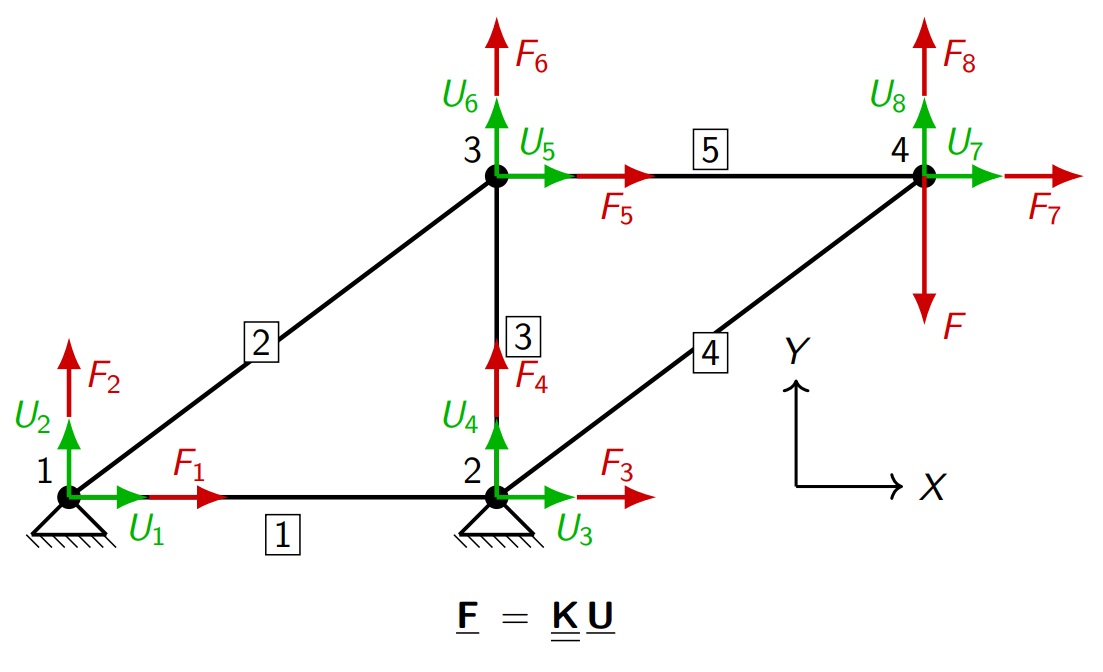
\includegraphics[width=\linewidth]{../Grafiken/Skizze.png}%

    \vfill
    \onslide<2->{%
      \text{Löse Gleichungssystem durch:}
      {\scriptsize
      \begin{align*}
        \fcolorbox{magenta!80!black}{white}{$\mathbf{F}_F$}
        &=
        \fcolorbox{orange!80!black}{white}{$\mathbf{K}_{FF}$}
        \fcolorbox{cyan!70!black}{white}{$\mathbf{U}_F$}
        +
        \fcolorbox{blue!70!black}{white}{$\mathbf{K}_{FU}$}
        \fcolorbox{purple!70!black}{white}{$\mathbf{U}_U$}
        \\
        \fcolorbox{teal!80!black}{white}{$\mathbf{F}_U$}
        &=
        \fcolorbox{red!80!black}{white}{$\mathbf{K}_{UF}$}
        \fcolorbox{cyan!70!black}{white}{$\mathbf{U}_F$}
        +
        \fcolorbox{green!60!black}{white}{$\mathbf{K}_{UU}$}
        \fcolorbox{purple!70!black}{white}{$\mathbf{U}_U$}
        \\
        \mathbf{U}_F &= \mathbf{K}_{FF}^{-1}\bigl(\mathbf{F}_F - \mathbf{K}_{FU}\mathbf{U}_U\bigr)\\
        \mathbf{F}_U &= \mathbf{K}_{UF}\mathbf{U}_F + \mathbf{K}_{UU}\mathbf{U}_U
      \end{align*}

      {\tiny Hinweis: Bei homogenen Randbedingungen (wie in diesem Beispiel) gilt $\mathbf{U}_U=\mathbf{0}$.}
      }%
    }
  \end{column}
  \begin{column}{0.74\textwidth}
    \centering
    \begin{tikzpicture}[
      ampersand replacement=\&,
      every node/.style={font=\scriptsize, anchor=center},
      knownF/.style={fill=orange!22, rounded corners=1pt, opacity=0.65},
      knownU/.style={fill=green!22,  rounded corners=1pt, opacity=0.65}
    ]
  % --- Linke Darstellung: F = K U ---
  \matrix (F) [matrix of math nodes, nodes in empty cells,
    row sep=0.45ex, column sep=0.6ex,
    nodes={inner sep=1.0pt, minimum height=1.45ex, minimum width=1.6em},
    left delimiter=(, right delimiter=)
  ]{
    F_1 \\
    F_2 \\
    0 \\
    F_4 \\
    0 \\
    0 \\
    0 \\
    {-F} \\
  };

  \node (eq1) [right=0.8em of F] {$=$};

  \matrix (K) [right=0.8em of eq1, matrix of math nodes, nodes in empty cells,
    row sep=0.45ex, column sep=0.55ex,
    nodes={inner sep=1.0pt, minimum height=1.45ex, minimum width=1.75em},
    left delimiter=(, right delimiter=)
  ]{
    K_{11} \& K_{12} \& K_{13} \& K_{14} \& K_{15} \& K_{16} \& K_{17} \& K_{18} \\
    K_{21} \& K_{22} \& K_{23} \& K_{24} \& K_{25} \& K_{26} \& K_{27} \& K_{28} \\
    K_{31} \& K_{32} \& K_{33} \& K_{34} \& K_{35} \& K_{36} \& K_{37} \& K_{38} \\
    K_{41} \& K_{42} \& K_{43} \& K_{44} \& K_{45} \& K_{46} \& K_{47} \& K_{48} \\
    K_{51} \& K_{52} \& K_{53} \& K_{54} \& K_{55} \& K_{56} \& K_{57} \& K_{58} \\
    K_{61} \& K_{62} \& K_{63} \& K_{64} \& K_{65} \& K_{66} \& K_{67} \& K_{68} \\
    K_{71} \& K_{72} \& K_{73} \& K_{74} \& K_{75} \& K_{76} \& K_{77} \& K_{78} \\
    K_{81} \& K_{82} \& K_{83} \& K_{84} \& K_{85} \& K_{86} \& K_{87} \& K_{88} \\
  };

  \matrix (U) [right=2.0em of K, matrix of math nodes, nodes in empty cells,
    row sep=0.45ex, column sep=0.6ex,
    nodes={inner sep=1.0pt, minimum height=1.45ex, minimum width=1.6em},
    left delimiter=(, right delimiter=)
  ]{
    0 \\
    0 \\
    U_3 \\
    0 \\
    U_5 \\
    U_6 \\
    U_7 \\
    U_8 \\
  };

  % Markierungen im Hintergrund (damit Zahlen/Symbole sichtbar bleiben)
  \begin{pgfonlayer}{background}
    \foreach \r in {3,5,6,7,8} {\node[knownF, fit=(F-\r-1), inner sep=0pt] {};}
    \foreach \r in {1,2,4}     {\node[knownU, fit=(U-\r-1), inner sep=0pt] {};}
  \end{pgfonlayer}
\end{tikzpicture}

\vspace{0.2em}

\centering
$\mathbf{F}=\mathbf{K}\mathbf{U}$

\vspace{0.2em}

\centering
\begin{tikzpicture}[
  ampersand replacement=\&,
  every node/.style={font=\scriptsize, anchor=center},
  knownF/.style={fill=orange!22, rounded corners=1pt, opacity=0.65},
  knownU/.style={fill=green!22,  rounded corners=1pt, opacity=0.65}
]
  % --- Permutierte / blockierte Darstellung ---
  \matrix (Fp) [matrix of math nodes, nodes in empty cells,
    row sep=0.45ex, column sep=0.6ex,
    nodes={inner sep=1.0pt, minimum height=1.45ex, minimum width=1.6em},
    left delimiter=(, right delimiter=)
  ]{
    0 \\
    0 \\
    0 \\
    0 \\
    {-F} \\
    F_1 \\
    F_2 \\
    F_4 \\
  };

  \node (eq2) [right=0.8em of Fp] {$=$};

  \matrix (Kp) [right=1.0em of eq2, matrix of math nodes, nodes in empty cells,
    row sep=0.45ex, column sep=0.55ex,
    nodes={inner sep=1.0pt, minimum height=1.45ex, minimum width=1.75em},
    left delimiter=(, right delimiter=)
  ]{
    K_{33} \& K_{35} \& K_{36} \& K_{37} \& K_{38} \& K_{31} \& K_{32} \& K_{34} \\
    K_{53} \& K_{55} \& K_{56} \& K_{57} \& K_{58} \& K_{51} \& K_{52} \& K_{54} \\
    K_{63} \& K_{65} \& K_{66} \& K_{67} \& K_{68} \& K_{61} \& K_{62} \& K_{64} \\
    K_{73} \& K_{75} \& K_{76} \& K_{77} \& K_{78} \& K_{71} \& K_{72} \& K_{74} \\
    K_{83} \& K_{85} \& K_{86} \& K_{87} \& K_{88} \& K_{81} \& K_{82} \& K_{84} \\
    K_{13} \& K_{15} \& K_{16} \& K_{17} \& K_{18} \& K_{11} \& K_{12} \& K_{14} \\
    K_{23} \& K_{25} \& K_{26} \& K_{27} \& K_{28} \& K_{21} \& K_{22} \& K_{24} \\
    K_{43} \& K_{45} \& K_{46} \& K_{47} \& K_{48} \& K_{41} \& K_{42} \& K_{44} \\
  };

  % Blockrahmen
  \draw[orange!80!black, line width=0.8pt] (Kp-1-1.north west) rectangle (Kp-5-5.south east);
  \draw[blue!70!black,   line width=0.8pt] (Kp-1-6.north west) rectangle (Kp-5-8.south east);
  \draw[red!80!black,    line width=0.8pt] (Kp-6-1.north west) rectangle (Kp-8-5.south east);
  \draw[green!60!black,  line width=0.8pt] (Kp-6-6.north west) rectangle (Kp-8-8.south east);

  \matrix (Up) [right=2.0em of Kp, matrix of math nodes, nodes in empty cells,
    row sep=0.45ex, column sep=0.6ex,
    nodes={inner sep=1.0pt, minimum height=1.45ex, minimum width=1.6em},
    left delimiter=(, right delimiter=)
  ]{
    U_3 \\
    U_5 \\
    U_6 \\
    U_7 \\
    U_8 \\
    0 \\
    0 \\
    0 \\
  };

  \begin{pgfonlayer}{background}
    % Kräfte: F_F (magenta), F_U (teal)
    \draw[magenta!80!black, line width=0.8pt] (Fp-1-1.north west) rectangle (Fp-5-1.south east);
    \draw[teal!80!black,    line width=0.8pt] (Fp-6-1.north west) rectangle (Fp-8-1.south east);

    % Verschiebungen: U_F (cyan), U_U (violett)
    \draw[cyan!70!black, line width=0.8pt] (Up-1-1.north west) rectangle (Up-5-1.south east);
    \draw[purple!70!black, line width=0.8pt] (Up-6-1.north west) rectangle (Up-8-1.south east);
\end{pgfonlayer}
\end{tikzpicture}
\end{column}
\end{columns}
\end{frame}

\begin{frame}{Ausblick: 1D-Stab-Element: Nachlaufrechnung}
  \centering
\begin{tikzpicture}[
    scale=0.58,
    every node/.style={font=\scriptsize},
    axis/.style={very thick, -{Latex[length=2.6mm]}},
    bar/.style={line width=1.8pt, black},
    joint/.style={circle, fill=blue!70, inner sep=2.2pt},
    uarr/.style={draw=green!70!black, very thick, -{Latex[length=2.6mm]}, green!70!black},
    farr/.style={draw=red!80!black,   very thick, -{Latex[length=2.6mm]}, red!80!black},
    dim/.style={thin, {Latex[length=2.3mm]}-{Latex[length=2.3mm]}}
  ]
    % Knotenkoordinaten
    \coordinate (n1) at (0,0);
    \coordinate (n2) at (8,0);

    % Stab
    \draw[bar] (n1) -- (n2);

    % Knotenpunkte
    \node[joint] at (n1) {};
    \node[joint] at (n2) {};

    % Knotennummern
    \node[blue!70!black, above right] at (n1) {\Large 1};
    \node[blue!70!black, above left] at (n2) {\Large 2};

    % Achsen (links y, rechts x) – mit Abstand zu den Knoten
    \draw[axis] ($(n1)+(0,0.15)$) -- ++(0,2.15) node[left] {$y$};
    \draw[axis] ($(n2)+(0.15,0)$) -- ++(2.45,0) node[below] {$x$};

    % Verschiebungen u^e (grün)
    \draw[uarr] (n1) ++(-1.6,-0.45) -- ++(1.6,0) node[midway, below] {$u_1^{e}$};
    \draw[uarr] (n2) ++(0.0,-0.45)  -- ++(1.6,0) node[midway, below] {$u_2^{e}$};

    % Knotenkräfte f^e (rot)
    \draw[farr] (n1) ++(-1.6,0.45) -- ++(1.6,0) node[midway, above] {$f_1^{e}$};
    \draw[farr] (n2) ++(0.0,0.45)  -- ++(1.6,0) node[midway, above] {$f_2^{e}$};

    % Material/Querschnitt
    \node[above] at ($(n1)!0.50!(n2)+(0,0.25)$) {$E^{e}A^{e}$};

    % L^e Dimension unten (mit Hilfslinien + Pfeile beidseitig)
    \draw[thin] (n1) -- ++(0,-1.0);
    \draw[thin] (n2) -- ++(0,-1.0);
    \draw[dim] ($(n1)+(0,-1.0)$) -- ($(n2)+(0,-1.0)$) node[midway, below] {$L^{e}$};
  \end{tikzpicture}

  \vspace{0.02em}

  % Formeln darunter
  \scriptsize
  \begin{align*}
    \text{Schritt 0: Globale Verschiebungen berechnet } \mathbf{U}&&
   \\
   \text{Schritt 1 (Wird noch näher behandelt): globale Elementverschiebungen berechnen}&&\mathbf{U}^{e} &= \mathbf{\hat{T}}^{e}\,\mathbf{U}
   \\
   \text{Schritt 2: lokale Elementverschiebungen berechnen}&&\mathbf{u}^{e} &= \mathbf{{T}}^{e}\mathbf{U}^{e} = \bigl(u^{e}_{1}\; u^{e}_{2}\bigr)^{T}
   \\
    \text{Schritt 2: Dehnung im Stab berechnen}&&\mathbf{\varepsilon}^{e} &= \frac{\Delta L^{e}}{L^{e}} =\frac{u^{e}_{2}-u^{e}_{1}}{L^{e}} 
    \\
    \text{Schritt 3: Spannung im Stab berechnen}&&\mathbf{\sigma}^{e} &= E^{e}\varepsilon^{e}
  \end{align*}
\end{frame}
\end{document}